\documentclass[letterpaper, 12pt]{article}
\usepackage[top=2cm,bottom=1cm,left=0.75in,right=0.75in,headheight=17pt, % as per the warning by fancyhdr
includehead,includefoot,
heightrounded, % to avoid spurious underfull messages
]{geometry}
\addtolength{\topmargin}{-.25in}
\usepackage{fancyhdr}
\pagestyle{fancy}
\usepackage{graphicx}
\usepackage{lastpage}
\usepackage{enumitem,amssymb}

\begin{document}
\fancyhead[l]{	\includegraphics[height=1cm]{"../../Templates/Year C/club".png} Name:}
\fancyhead[r]{Due Date \hspace{ 1in}}
\cfoot{\thepage\ of \pageref{LastPage}}
	

	
\begin{center}Assignment 5.01: Magnetic Force on Particles
\end{center}

\begin{enumerate}
	\item  Identify the direction of the magnetic force on each particle.  Draw an arrow to represent the direction of the force.
	
	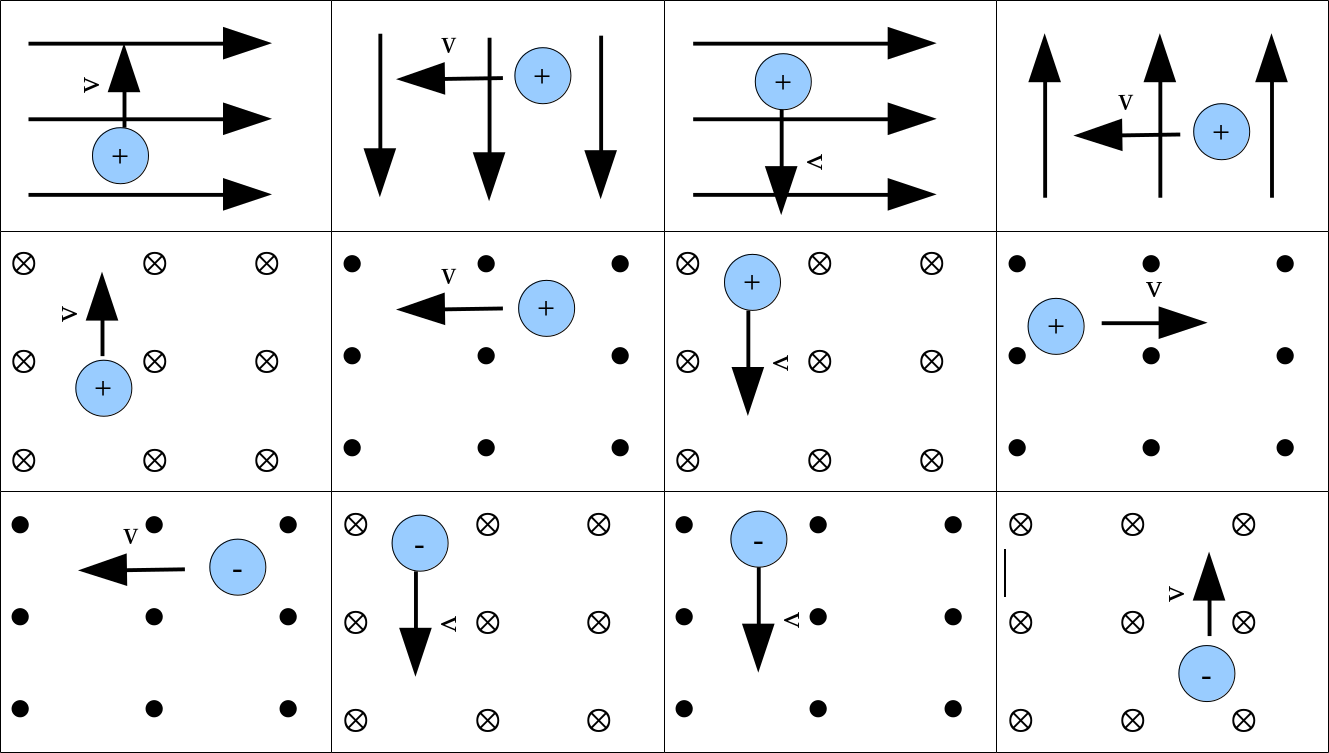
\includegraphics[height=3.5in]{../particlesinmagneticfields.png}
	
	\item An electron is moving to the left at 3 m/s.  It is in a 0.25 T magnetic field, directed out of the page. What is the force on the electron?  (Magnitude and direction).
	\vspace{1in}

	\item A proton is traveling at 200 m/s to the right in a 1.2 T magnetic field directed into the page.  
		\begin{enumerate}
			\item What is the force the proton experiences?
			\vspace{.75in}
			\item What is the radius of the circle that the proton travels in?
		\end{enumerate}
	
	\vspace{.9in}
	
	\item  A magnetic field is directed to the southeast, with a magnitude of 0.125 T.  A particle travels to the north at 43000 m/s.  What is the magnetic force (magnitude and direction) on the particle?
	
	\vspace{1in}
	\item Pikachu, on the left, wants to attack his opponent, Magnetmite, on the right.  Pikachu has an electrical charge of 2.5 C. Magnetmite directs his magnetic field toward Pikachu.  
		\begin{enumerate}
			\vspace{-.05in}
			\item What moves will be the best for Pikachu to do to eliminate Magnetmite's attack? (check any that apply)
			
			\begin{large}
				$\square $ 
			\end{large} 
			Circle around and charge-attack from the side.
			
			\begin{large}
				$\square $ 
			\end{large} 
			Sidestep, then charge-attack.
			
			\begin{large}
				$\square $ 
			\end{large} 
			Run directly toward Magnetmite, and use Volt-Tackle
		
			\begin{large}
				$\square $ 
			\end{large} 
			Jump upward, then use Lightning-bolt.
	
			\begin{large}
				$\square $ 
			\end{large} 
			Stay still and wait for Magnetmite to turn off his magnetic field.

			\item Explain your answer.
			\vspace{.9in}
			
			
			
		\end{enumerate}
		
		\item In an experiment, a proton passes through a 1.5 T magnetic field.  The proton moves through the magnetic field in an unknown direction at a speed of 6 x 10\textsuperscript{6} m/s.  
		\begin{enumerate}
			\item a) Calculate the minimum possible force exerted on the proton.
			\vspace{.4in}
			
			\item Calculate the maximum possible force exerted on the proton.
			\vspace{.4in}
			
			
			\item Calculate the maximum possible acceleration of the proton.
			
				\vspace{.4in}
			
			\item Would an electron moving through the field experience the same maximum force?
				\vspace{.4in}
			
			\item Would an electron's maximum possible acceleration be the same as the proton's maximum possible acceleration? 
			
		\end{enumerate}
	


	
\end{enumerate}
 



\end{document}
